\section{Физическое кодирование}
\subsection{NRZ}
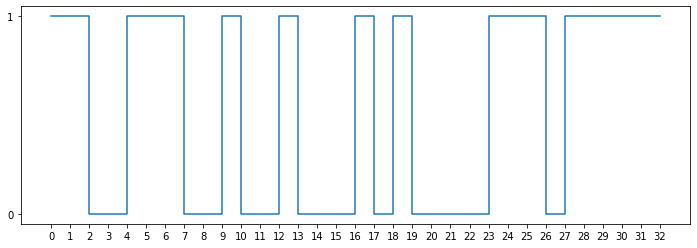
\includegraphics[width=\textwidth]{3nrz}

Минимальный интервал (все сообщение): $t_\mathrm{min}=1.0$ битовых интервалов

Максимальный интервал (все сообщение): $t_\mathrm{max}=4.0$ битовых интервалов

Максимальная частота: $f_\mathrm{max}=C\div t_\mathrm{min}=1000.0\div 2=500.0$ МГц

Минимальная частота: $f_\mathrm{min}=C\div t_\mathrm{max}=1000.0\div 8=125.0$ МГц

Полоса пропускания: $S=7f_\mathrm{max}-f_\mathrm{min} = 7\cdot 500.0\text{ МГц}-125.0\text{ МГц}=3375.0$ МГц

Количество интервалов с одинаковым уровнем (все сообщение): $n_\mathrm{similar}=52$

Время передачи сообщения: $T=88.0$ битовых интервалов

Среднее: $f_0\cdot n_\mathrm{similar}\div T=1000.0\text{ МГц}\cdot 26.0\div 88.0=295.5$ МГц

\subsection{RZ}
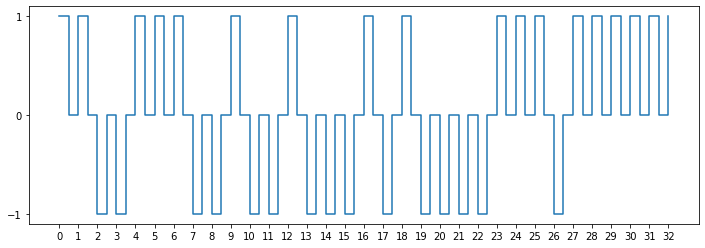
\includegraphics[width=\textwidth]{3rz}

Минимальный интервал (все сообщение): $t_\mathrm{min}=0.5$ битовых интервалов

Максимальный интервал (все сообщение): $t_\mathrm{max}=1.0$ битовых интервалов

Максимальная частота: $f_\mathrm{max}=C\div t_\mathrm{min}=1000.0\div 1=1000.0$ МГц

Минимальная частота: $f_\mathrm{min}=C\div t_\mathrm{max}=1000.0\div 2=500.0$ МГц

Полоса пропускания: $S=7f_\mathrm{max}-f_\mathrm{min} = 7\cdot 1000.0\text{ МГц}-500.0\text{ МГц}=6500.0$ МГц

Количество интервалов с одинаковым уровнем (все сообщение): $n_\mathrm{similar}=176$

Время передачи сообщения: $T=88.0$ битовых интервалов

Среднее: $f_0\cdot n_\mathrm{similar}\div T=1000.0\text{ МГц}\cdot 88.0\div 88.0=1000.0$ МГц

\subsection{AMI}
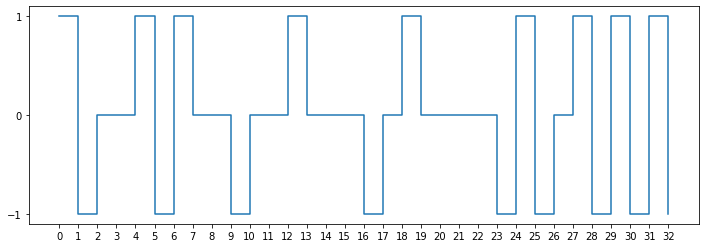
\includegraphics[width=\textwidth]{3ami}

Минимальный интервал (все сообщение): $t_\mathrm{min}=1.0$ битовых интервалов

Максимальный интервал (все сообщение): $t_\mathrm{max}=3.0$ битовых интервалов

Максимальная частота: $f_\mathrm{max}=C\div t_\mathrm{min}=1000.0\div 2=500.0$ МГц

Минимальная частота: $f_\mathrm{min}=C\div t_\mathrm{max}=1000.0\div 6=166.7$ МГц

Полоса пропускания: $S=7f_\mathrm{max}-f_\mathrm{min} = 7\cdot 500.0\text{ МГц}-166.7\text{ МГц}=3333.3$ МГц

Количество интервалов с одинаковым уровнем (все сообщение): $n_\mathrm{similar}=75$

Время передачи сообщения: $T=88.0$ битовых интервалов

Среднее: $f_0\cdot n_\mathrm{similar}\div T=1000.0\text{ МГц}\cdot 37.5\div 88.0=426.1$ МГц

\subsection{NRZI}
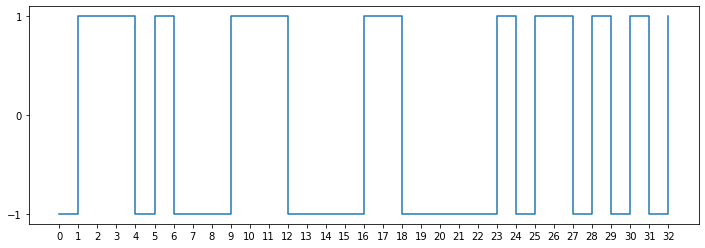
\includegraphics[width=\textwidth]{3nrzi}

Минимальный интервал (все сообщение): $t_\mathrm{min}=1.0$ битовых интервалов

Максимальный интервал (все сообщение): $t_\mathrm{max}=4.0$ битовых интервалов

Максимальная частота: $f_\mathrm{max}=C\div t_\mathrm{min}=1000.0\div 2=500.0$ МГц

Минимальная частота: $f_\mathrm{min}=C\div t_\mathrm{max}=1000.0\div 8=125.0$ МГц

Полоса пропускания: $S=7f_\mathrm{max}-f_\mathrm{min} = 7\cdot 500.0\text{ МГц}-125.0\text{ МГц}=3375.0$ МГц

Количество интервалов с одинаковым уровнем (все сообщение): $n_\mathrm{similar}=49$

Время передачи сообщения: $T=88.0$ битовых интервалов

Среднее: $f_0\cdot n_\mathrm{similar}\div T=1000.0\text{ МГц}\cdot 24.5\div 88.0=278.4$ МГц

\subsection{Манчестерский код}
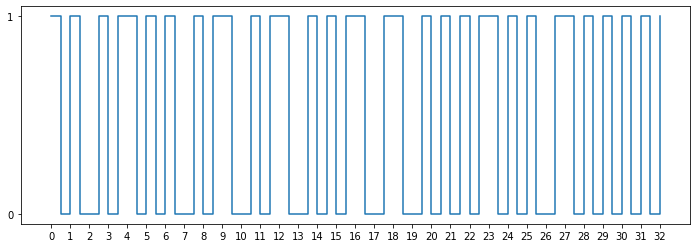
\includegraphics[width=\textwidth]{3manchester}

Минимальный интервал (все сообщение): $t_\mathrm{min}=0.5$ битовых интервалов

Максимальный интервал (все сообщение): $t_\mathrm{max}=1.0$ битовых интервалов

Максимальная частота: $f_\mathrm{max}=C\div t_\mathrm{min}=1000.0\div 1=1000.0$ МГц

Минимальная частота: $f_\mathrm{min}=C\div t_\mathrm{max}=1000.0\div 2=500.0$ МГц

Полоса пропускания: $S=7f_\mathrm{max}-f_\mathrm{min} = 7\cdot 1000.0\text{ МГц}-500.0\text{ МГц}=6500.0$ МГц

Количество интервалов с одинаковым уровнем (все сообщение): $n_\mathrm{similar}=125$

Время передачи сообщения: $T=88.0$ битовых интервалов

Среднее: $f_0\cdot n_\mathrm{similar}\div T=1000.0\text{ МГц}\cdot 62.5\div 88.0=710.2$ МГц

\subsection{Дифференциальный манчестерский код}
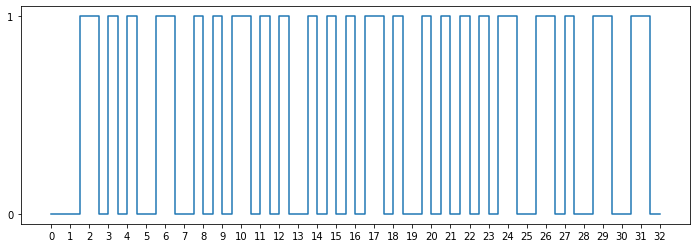
\includegraphics[width=\textwidth]{3manchester_diff}


Минимальный интервал (все сообщение): $t_\mathrm{min}=0.5$ битовых интервалов

Максимальный интервал (все сообщение): $t_\mathrm{max}=2.0$ битовых интервалов

Максимальная частота: $f_\mathrm{max}=C\div t_\mathrm{min}=1000.0\div 1=1000.0$ МГц

Минимальная частота: $f_\mathrm{min}=C\div t_\mathrm{max}=1000.0\div 4=250.0$ МГц

Полоса пропускания: $S=7f_\mathrm{max}-f_\mathrm{min} = 7\cdot 1000.0\text{ МГц}-250.0\text{ МГц}=6750.0$ МГц

Количество интервалов с одинаковым уровнем (все сообщение): $n_\mathrm{similar}=128$

Время передачи сообщения: $T=90.0$ битовых интервалов

Среднее: $f_0\cdot n_\mathrm{similar}\div T=1000.0\text{ МГц}\cdot 64.0\div 90.0=711.1$ МГц

\subsection{MLT-3}
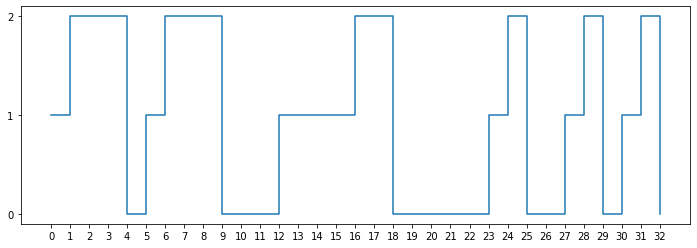
\includegraphics[width=\textwidth]{3mlt3}

Минимальный интервал (все сообщение): $t_\mathrm{min}=1.0$ битовых интервалов

Максимальный интервал (все сообщение): $t_\mathrm{max}=4.0$ битовых интервалов

Максимальная частота: $f_\mathrm{max}=C\div t_\mathrm{min}=1000.0\div 2=500.0$ МГц

Минимальная частота: $f_\mathrm{min}=C\div t_\mathrm{max}=1000.0\div 8=125.0$ МГц

Полоса пропускания: $S=7f_\mathrm{max}-f_\mathrm{min} = 7\cdot 500.0\text{ МГц}-125.0\text{ МГц}=3375.0$ МГц

Количество интервалов с одинаковым уровнем (все сообщение): $n_\mathrm{similar}=49$

Время передачи сообщения: $T=88.0$ битовых интервалов

Среднее: $f_0\cdot n_\mathrm{similar}\div T=1000.0\text{ МГц}\cdot 24.5\div 88.0=278.4$ МГц

\subsection{PAM-5}
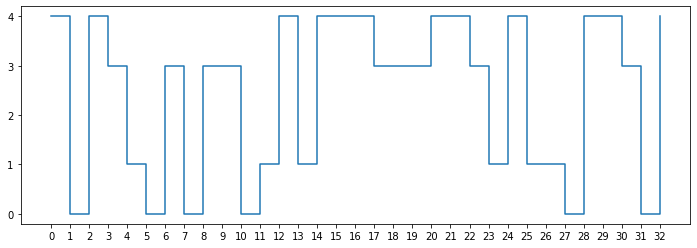
\includegraphics[width=\textwidth]{3pam5}

Минимальный интервал (все сообщение): $t_\mathrm{min}=1.0$ битовых интервалов

Максимальный интервал (все сообщение): $t_\mathrm{max}=3.0$ битовых интервалов

Максимальная частота: $f_\mathrm{max}=C\div t_\mathrm{min}=1000.0\div 2=500.0$ МГц

Минимальная частота: $f_\mathrm{min}=C\div t_\mathrm{max}=1000.0\div 6=166.7$ МГц

Полоса пропускания: $S=7f_\mathrm{max}-f_\mathrm{min} = 7\cdot 500.0\text{ МГц}-166.7\text{ МГц}=3333.3$ МГц

Количество интервалов с одинаковым уровнем (все сообщение): $n_\mathrm{similar}=34$

Время передачи сообщения: $T=44.0$ битовых интервалов

Среднее: $f_0\cdot n_\mathrm{similar}\div T=1000.0\text{ МГц}\cdot 17.0\div 44.0=386.4$ МГц

\subsection{Выбор лучшего}
\begin{center}
    \begin{tabular}{c|cccc}
        & $f_\mathrm{\text{в}}$, МГц
        & $f_\mathrm{\text{н}}$, МГц
        & $f_\mathrm{\text{с}}$, МГц
        & $S$, МГц \\ \hline
        NRZ               &  500.0 &  62.5 &  295.5 & 3437.5 \\
        RZ                & 1000.0 & 500.0 & 1000.0 & 6500.0 \\
        AMI               &  500.0 & 125.0 &  426.1 & 3375.0 \\
        NRZI              &  500.0 & 100.0 &  278.4 & 3400.0 \\
        Манчестерский код & 1000.0 & 500.0 &  710.2 & 6500.0 \\
        Дифф. манч. код   & 1000.0 & 250.0 &  711.1 & 6750.0 \\
        MLT-3             &  500.0 & 100.0 &  278.4 & 3400.0 \\
        PAM-5             &  500.0 & 166.7 &  386.4 & 3333.3 \\
    \end{tabular}
\end{center}

\begin{center}
    \begin{tabular}{c|cccc}
        & $S$, МГц
        & Уровни
        & Самосинхронизация
        & Обработка ошибок \\ \hline
        NRZ               & 3437.5 & 2 & - & - \\
        RZ                & 6500.0 & 3 & + & - \\
        AMI               & 3375.0 & 3 & - & + \\
        NRZI              & 3400.0 & 2 & - & - \\
        Манчестерский код & 6500.0 & 2 & + & - \\
        Дифф. манч. код   & 6750.0 & 2 & - & + \\
        MLT-3             & 3400.0 & 3 & - & - \\
        PAM-5             & 3333.3 & 5 & - & + \\
    \end{tabular}
\end{center}

Таким образом, оптимальными являются NRZ и NRZI --- несмотря на отсутствие самосинхронизации,
они обладают наименьшей необходимой полосой пропускания для минимального количества уровней сигнала.
Также хорошим выбором являются обычный и дифференциальный манчестерский код, т.к.
один имеет самосинхронизацию, а другой --- компенсацию ошибок, и оба также имеют лишь 2 уровня сигнала,
но они требуют гораздо более широкой полосы пропускания.
